\documentclass[tikz,border=1pt]{standalone}
\usepackage{tikz}
\usetikzlibrary{arrows.meta,shapes.geometric}
\definecolor{ink}{HTML}{222831}
\definecolor{steel}{HTML}{6B7C8C}
\definecolor{teal}{HTML}{6E8C8A}
\definecolor{gold}{HTML}{B08D57}
\definecolor{pale}{HTML}{EEF1F4}
\definecolor{field}{HTML}{E9EFF6}
\definecolor{iconbg}{HTML}{D8E0E4}
\begin{document}
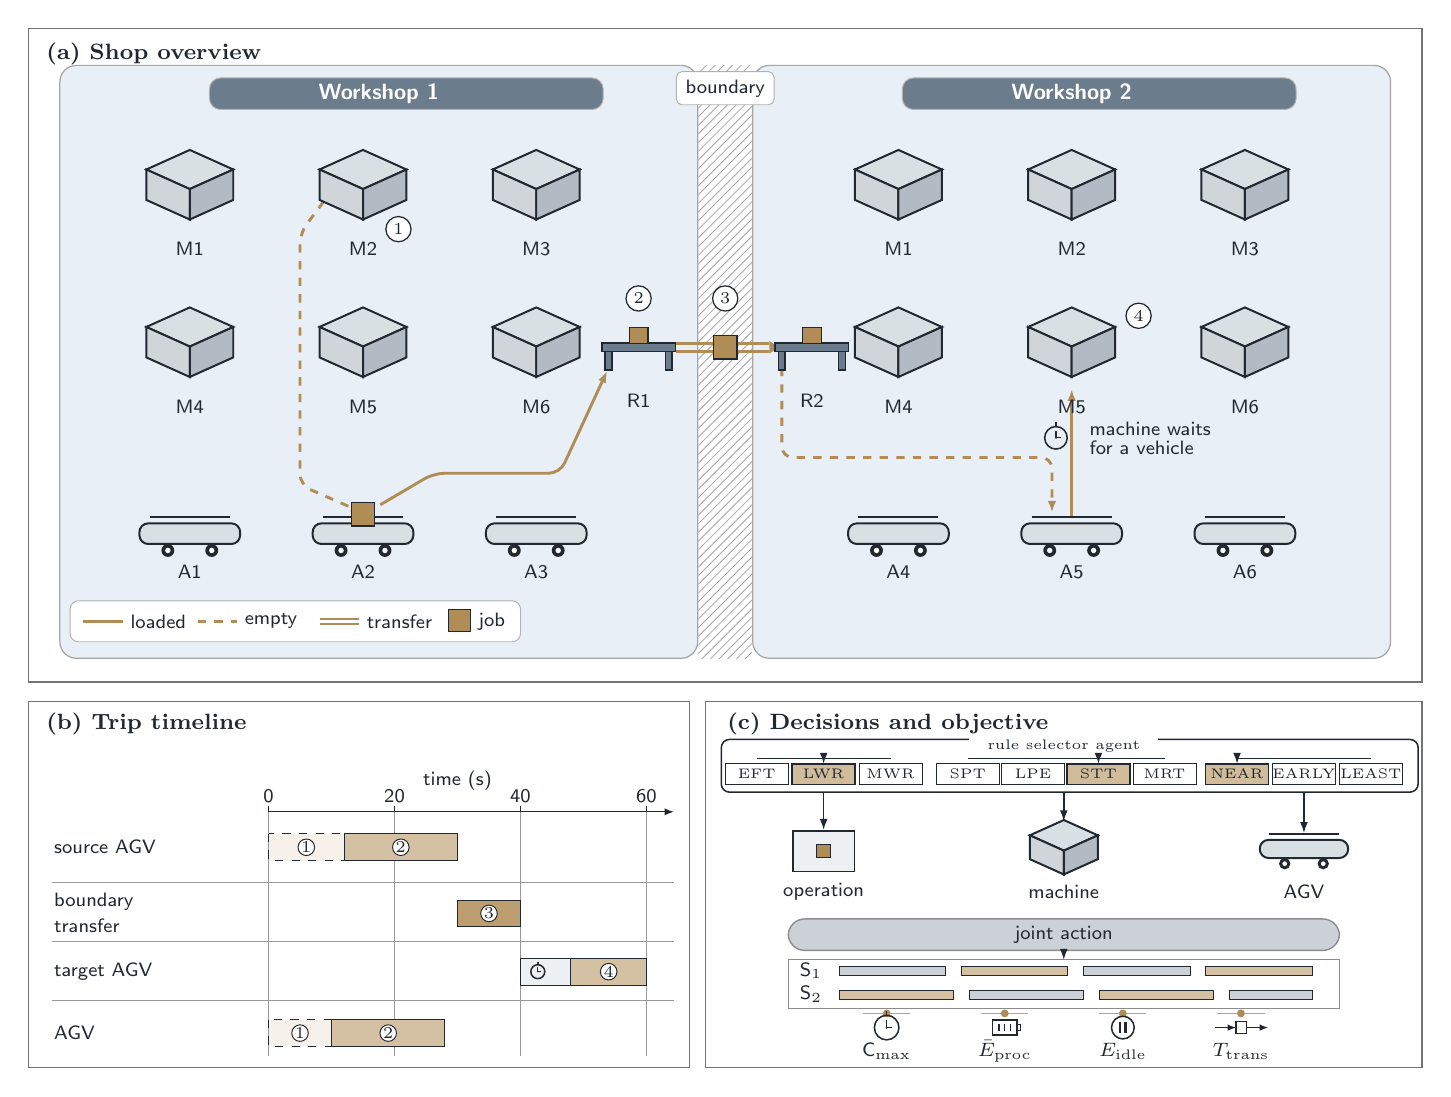
\begin{tikzpicture}[y=-1cm,x=1cm,font=\sffamily\fontsize{7.5}{9.2}\selectfont,
  every node/.style={inner sep=0.6pt},
  ar/.style={-{Latex[length=1.4mm,width=1.0mm]},line width=0.55pt,draw=ink},
  route/.style={gold,line width=1.05pt,rounded corners=4pt},
  routea/.style={route,-{Latex[length=1.5mm,width=1.1mm]}},
  panel/.style={draw=black!55,line width=0.5pt,fill=white},
  lab/.style={text=ink},
  title/.style={lab,anchor=west,font=\bfseries\fontsize{8.4}{10}\selectfont},
]

\tikzset{
  pics/machine/.style={code={\begin{scope}[yscale=-1]
    \fill[iconbg,draw=ink,line width=0.72pt]
      (0,0.55) -- (0.60,0.28) -- (0,0.01) -- (-0.60,0.28) -- cycle;
    \fill[steel!32!white,draw=ink,line width=0.72pt]
      (-0.60,0.28) -- (0,0.01) -- (0,-0.41) -- (-0.60,-0.14) -- cycle;
    \fill[steel!52!white,draw=ink,line width=0.72pt]
      (0,0.01) -- (0.60,0.28) -- (0.60,-0.14) -- (0,-0.41) -- cycle;
  \end{scope}}},
  pics/agv/.style={code={\begin{scope}[yscale=-1]
    \fill[fill=iconbg,draw=ink,line width=0.72pt,rounded corners=3.2pt]
      (-0.78,-0.12) rectangle (0.78,0.20);
    \draw[ink,line width=0.6pt] (-0.62,0.30) -- (0.62,0.30);
    \fill[ink] (-0.34,-0.22) circle (0.10);
    \fill[white] (-0.34,-0.22) circle (0.042);
    \fill[ink] (0.34,-0.22) circle (0.10);
    \fill[white] (0.34,-0.22) circle (0.042);
  \end{scope}}},
  pics/station/.style={code={\begin{scope}[yscale=-1]
    \fill[steel,draw=ink,line width=0.55pt] (-0.55,-0.06) rectangle (0.55,0.06);
    \fill[steel,draw=ink,line width=0.50pt] (-0.50,-0.06) rectangle (-0.40,-0.34);
    \fill[steel,draw=ink,line width=0.50pt] (0.40,-0.06) rectangle (0.50,-0.34);
    \fill[gold,draw=ink,line width=0.45pt] (-0.14,0.06) rectangle (0.14,0.30);
  \end{scope}}},
  pics/job/.style={code={\begin{scope}[yscale=-1]
    \fill[gold,draw=ink,line width=0.45pt] (-0.15,-0.15) rectangle (0.15,0.15);
  \end{scope}}},
  pics/switch/.style={code={\begin{scope}[yscale=-1]
    \fill[white,draw=ink,line width=0.6pt,rounded corners=1.6pt]
      (-0.62,-0.34) rectangle (0.62,0.34);
    \draw[ink,line width=0.5pt] (0,-0.34) -- (0,-0.16);
    \fill[ink] (0,-0.16) circle (0.055);
    \fill[ink] (-0.38,0.22) circle (0.055);
    \fill[ink] (0.00,0.26) circle (0.055);
    \fill[ink] (0.38,0.22) circle (0.055);
    \draw[gold,line width=1.2pt] (0,-0.16) -- (-0.36,0.19);
  \end{scope}}},
  pics/switch4/.style={code={\begin{scope}[yscale=-1]
    \fill[white,draw=ink,line width=0.6pt,rounded corners=1.6pt]
      (-0.62,-0.34) rectangle (0.62,0.34);
    \draw[ink,line width=0.5pt] (0,-0.34) -- (0,-0.16);
    \fill[ink] (0,-0.16) circle (0.055);
    \fill[ink] (-0.45,0.20) circle (0.055);
    \fill[ink] (-0.15,0.26) circle (0.055);
    \fill[ink] (0.15,0.26) circle (0.055);
    \fill[ink] (0.45,0.20) circle (0.055);
    \draw[gold,line width=1.2pt] (0,-0.16) -- (-0.43,0.17);
  \end{scope}}},
  pics/operation/.style={code={\begin{scope}[yscale=-1]
    \fill[pale,draw=ink,line width=0.55pt] (-0.46,-0.30) rectangle (0.46,0.30);
    \fill[gold,draw=ink,line width=0.35pt] (-0.10,-0.10) rectangle (0.10,0.10);
  \end{scope}}},
  pics/clock/.style={code={\begin{scope}[yscale=-1]
    \draw[ink,line width=0.55pt] (0,0) circle (0.26);
    \draw[ink,line width=0.55pt] (0,0.26) -- (0,0.36);
    \draw[ink,line width=0.45pt] (0,0) -- (0,0.16);
    \draw[ink,line width=0.45pt] (0,0) -- (0.12,0.00);
    \fill[ink] (0,0) circle (0.025);
  \end{scope}}},
  pics/battery/.style={code={\begin{scope}[yscale=-1]
    \draw[ink,line width=0.55pt,fill=white] (-0.26,-0.16) rectangle (0.26,0.16);
    \draw[ink,line width=0.45pt] (0.26,-0.06) -- (0.34,-0.06) -- (0.34,0.06) -- (0.26,0.06);
    \draw[ink,line width=0.45pt] (-0.12,-0.08) -- (-0.12,0.08);
    \draw[ink,line width=0.45pt] (0.00,-0.08) -- (0.00,0.08);
    \draw[ink,line width=0.45pt] (0.12,-0.08) -- (0.12,0.08);
  \end{scope}}},
  pics/pause/.style={code={\begin{scope}[yscale=-1]
    \draw[ink,line width=0.55pt,fill=white] (0,0) circle (0.24);
    \fill[ink] (-0.09,-0.11) rectangle (-0.03,0.11);
    \fill[ink] (0.03,-0.11) rectangle (0.09,0.11);
  \end{scope}}},
  pics/tec/.style={code={\begin{scope}[yscale=-1]
    \draw[ink,line width=0.55pt,fill=white] (-0.10,-0.13) rectangle (0.12,0.13);
    \draw[ink,line width=0.5pt,-{Latex[length=1.1mm]}] (-0.56,0.00) -- (-0.10,0.00);
    \draw[ink,line width=0.5pt,-{Latex[length=1.1mm]}] (0.12,0.00) -- (0.58,0.00);
  \end{scope}}},
}

% ---------------- frames ----------------
\draw[panel] (0.15,0.15) rectangle (17.85,8.45);
\draw[panel] (0.15,8.70) rectangle (8.55,13.35);
\draw[panel] (8.75,8.70) rectangle (17.85,13.35);

% ================= (a) =================
\node[title] at (0.35,0.47) {(a) Shop overview};

\draw[black!35,line width=0.45pt,fill=field,rounded corners=6pt]
  (0.55,0.62) rectangle (8.65,8.15);
\draw[black!35,line width=0.45pt,fill=field,rounded corners=6pt]
  (9.35,0.62) rectangle (17.45,8.15);
\begin{scope}
  \clip (8.66,0.62) rectangle (9.34,8.15);
  \foreach \k in {-1.0,-0.89,...,9.4} {
    \draw[black!35,line width=0.3pt] (8.40,\k) -- (9.60,\k-1.20);
  }
\end{scope}
\draw[black!30,line width=0.35pt,fill=white,rounded corners=2pt]
  (8.38,0.70) rectangle (9.62,1.12);
\node[lab] at (9.00,0.91) {boundary};

\draw[black!30,line width=0.35pt,fill=steel,rounded corners=4pt]
  (2.45,0.78) rectangle (7.45,1.18);
\node[white] at (4.60,0.98)
  {\bfseries\fontsize{7.8}{9.4}\selectfont Workshop 1};
\draw[black!30,line width=0.35pt,fill=steel,rounded corners=4pt]
  (11.25,0.78) rectangle (16.25,1.18);
\node[white] at (13.40,0.98)
  {\bfseries\fontsize{7.8}{9.4}\selectfont Workshop 2};

% route first
\draw[routea,dashed] (3.90,2.35) -- (3.60,2.75) -- (3.60,3.65) --
  (3.60,5.95) -- (4.4,6.30);
\draw[routea] (4.62,6.20) -- (5.30,5.80) -- (6.90,5.80) -- (7.50,4.50);
\draw[gold,line width=0.95pt] (8.37,4.15) -- (9.56,4.15);
\draw[gold,line width=0.95pt] (8.37,4.25) -- (9.56,4.25);
\fill[gold] (9.56,4.12) -- (9.56,4.28) -- (9.68,4.20) -- cycle;
\draw[routea,dashed] (9.72,4.46) -- (9.72,5.60) -- (13.15,5.60) -- (13.15,6.30);
\draw[routea] (13.4,6.35) -- (13.4,4.73);

% machines
\foreach \xx in {2.2,4.4,6.6} {
  \foreach \yy in {2.20,4.20} { \pic[scale=0.92] at (\xx,\yy) {machine}; }
}
\foreach \xx in {11.2,13.4,15.6} {
  \foreach \yy in {2.20,4.20} { \pic[scale=0.92] at (\xx,\yy) {machine}; }
}
\node[lab] at (2.2,2.95) {M1}; \node[lab] at (4.4,2.95) {M2}; \node[lab] at (6.6,2.95) {M3};
\node[lab] at (2.2,4.95) {M4}; \node[lab] at (4.4,4.95) {M5}; \node[lab] at (6.6,4.95) {M6};
\node[lab] at (11.2,2.95) {M1}; \node[lab] at (13.4,2.95) {M2}; \node[lab] at (15.6,2.95) {M3};
\node[lab] at (11.2,4.95) {M4}; \node[lab] at (13.4,4.95) {M5}; \node[lab] at (15.6,4.95) {M6};

% stations
\pic[scale=0.85] at (7.90,4.20) {station}; \node[lab] at (7.90,4.88) {R1};
\pic[scale=0.85] at (10.10,4.20) {station}; \node[lab] at (10.10,4.88) {R2};

% AGVs
\foreach \xx/\nn in {2.2/A1,4.4/A2,6.6/A3} {
  \pic[scale=0.82] at (\xx,6.60) {agv}; \node[lab] at (\xx,7.05) {\nn};
}
\foreach \xx/\nn in {11.2/A4,13.4/A5,15.6/A6} {
  \pic[scale=0.82] at (\xx,6.60) {agv}; \node[lab] at (\xx,7.05) {\nn};
}

% jobs
\pic at (4.4,6.32) {job};
\pic at (9.00,4.20) {job};

% step numbers
\foreach \x/\y/\n in {4.85/2.70/1, 7.90/3.58/2, 9.00/3.58/3, 14.25/3.80/4} {
  \fill[white,draw=ink,line width=0.45pt] (\x,\y) circle (0.16);
  \node[lab,font=\fontsize{6.2}{7.2}\selectfont] at (\x,\y) {\n};
}

% callout
\pic[scale=0.55] at (13.20,5.35) {clock};
\node[lab,anchor=west] at (13.60,5.23) {machine waits};
\node[lab,anchor=west] at (13.60,5.48) {for a vehicle};

% legend
\draw[black!30,line width=0.35pt,fill=white,rounded corners=3pt]
  (0.68,7.42) rectangle (6.40,7.94);
\draw[route] (0.85,7.68) -- (1.35,7.68);
\node[lab,anchor=west] at (1.42,7.68) {loaded};
\draw[route,dashed] (2.30,7.68) -- (2.80,7.68);
\node[lab,anchor=west] at (2.87,7.68) {empty};
\draw[gold,line width=0.7pt] (3.85,7.65) -- (4.35,7.65);
\draw[gold,line width=0.7pt] (3.85,7.71) -- (4.35,7.71);
\node[lab,anchor=west] at (4.42,7.68) {transfer};
\fill[gold,draw=ink,line width=0.4pt] (5.48,7.53) rectangle (5.76,7.81);
\node[lab,anchor=west] at (5.84,7.68) {job};

% ================= (b) =================
\node[title] at (0.35,8.98) {(b) Trip timeline};

\draw[ink,line width=0.45pt,-{Latex[length=1.2mm]}] (3.2,10.10) -- (8.35,10.10);
\foreach \x/\t in {3.2/0,4.8/20,6.4/40,8.0/60} {
  \draw[black!40,line width=0.35pt] (\x,10.10) -- (\x,13.20);
  \draw[ink,line width=0.35pt] (\x,10.10) -- (\x,10.02);
  \node[lab] at (\x,9.90) {\t};
}
\node[lab] at (5.6,9.70) {time (s)};
\draw[black!40,line width=0.35pt] (0.45,11.00) -- (8.35,11.00);
\draw[black!40,line width=0.35pt] (0.45,11.75) -- (8.35,11.75);
\draw[black!40,line width=0.35pt] (0.45,12.50) -- (8.35,12.50);

\node[lab,anchor=west] at (0.45,10.55) {source AGV};
\node[lab,anchor=west,align=left] at (0.45,11.38) {boundary\\transfer};
\node[lab,anchor=west] at (0.45,12.13) {target AGV};
\node[lab,anchor=west] at (0.45,12.90) {AGV};

\draw[ink,line width=0.35pt,dashed,fill=gold!12!white] (3.20,10.38) rectangle (4.16,10.72);
\fill[gold!55!white,draw=ink,line width=0.35pt] (4.16,10.38) rectangle (5.60,10.72);

\fill[gold!85!white,draw=ink,line width=0.35pt] (5.60,11.22) rectangle (6.40,11.56);

\fill[pale,draw=ink,line width=0.35pt] (6.40,11.96) rectangle (7.04,12.30);
\pic[scale=0.34] at (6.62,12.13) {clock};
\fill[gold!55!white,draw=ink,line width=0.35pt] (7.04,11.96) rectangle (8.00,12.30);

\draw[ink,line width=0.35pt,dashed,fill=gold!12!white] (3.20,12.74) rectangle (4.00,13.08);
\fill[gold!55!white,draw=ink,line width=0.35pt] (4.00,12.74) rectangle (5.44,13.08);

\foreach \x/\y/\n in {3.68/10.55/1,4.88/10.55/2,6.00/11.39/3,7.52/12.13/4,3.60/12.91/1,4.72/12.91/2} {
  \fill[white,draw=ink,line width=0.35pt] (\x,\y) circle (0.105);
  \node[lab,font=\fontsize{6.0}{7.2}\selectfont] at (\x,\y) {\n};
}

% ================= (c) =================
\node[title] at (9.00,8.98) {(c) Decisions and objective};

\draw[ink,line width=0.55pt,rounded corners=3pt,fill=white]
  (8.95,9.18) rectangle (17.80,9.85);
\fill[white] (12.10,9.14) rectangle (14.50,9.40);
\node[lab,font=\fontsize{5.4}{6.6}\selectfont] at (13.30,9.27) {rule selector agent};
\draw[ink,line width=0.45pt] (9.40,9.42) -- (11.10,9.42);
\draw[ink,line width=0.45pt] (12.08,9.42) -- (14.58,9.42);
\draw[ink,line width=0.45pt] (15.50,9.42) -- (17.20,9.42);
\draw[ar] (10.25,9.42) -- (10.25,9.49);
\draw[ar] (13.74,9.42) -- (13.74,9.49);
\draw[ar] (15.50,9.42) -- (15.50,9.49);

\foreach \x/\t/\sel in {9.40/EFT/0,10.25/LWR/1,11.10/MWR/0,
  12.08/SPT/0,12.91/LPE/0,13.74/STT/1,14.58/MRT/0,
  15.50/NEAR/1,16.35/EARLY/0,17.20/LEAST/0} {
  \ifnum\sel=1
    \fill[gold!60!white,draw=ink,line width=0.5pt] (\x-0.40,9.49) rectangle (\x+0.40,9.75);
  \else
    \fill[white,draw=ink,line width=0.4pt] (\x-0.40,9.49) rectangle (\x+0.40,9.75);
  \fi
  \node[lab,font=\fontsize{5.0}{6.2}\selectfont] at (\x,9.62) {\t};
}

\pic[scale=0.85] at (10.25,10.60) {operation};
\pic[scale=0.72] at (13.30,10.60) {machine};
\pic[scale=0.72] at (16.35,10.60) {agv};
\node[lab] at (10.25,11.11) {operation};
\node[lab] at (13.30,11.11) {machine};
\node[lab] at (16.35,11.11) {AGV};

\draw[ar] (10.25,9.85) -- (10.25,10.33);
\draw[ar] (13.30,9.85) -- (13.30,10.22);
\draw[ar] (16.35,9.85) -- (16.35,10.37);

\draw[black!45,line width=0.5pt,fill=steel!35!white,rounded corners=6pt]
  (9.80,11.46) rectangle (16.80,11.86);
\node[lab] at (13.30,11.66) {joint action};

\draw[ar] (13.30,11.86) -- (13.30,11.98);

\draw[black!45,line width=0.4pt] (9.80,11.98) rectangle (16.80,12.60);
\node[lab,anchor=west] at (9.92,12.12) {S$_1$};
\node[lab,anchor=west] at (9.92,12.42) {S$_2$};
\fill[steel!35!white,draw=ink,line width=0.2pt] (10.45,12.06) rectangle (11.80,12.18);
\fill[gold!55!white,draw=ink,line width=0.2pt] (12.00,12.06) rectangle (13.35,12.18);
\fill[steel!35!white,draw=ink,line width=0.2pt] (13.55,12.06) rectangle (14.90,12.18);
\fill[gold!55!white,draw=ink,line width=0.2pt] (15.10,12.06) rectangle (16.45,12.18);
\fill[gold!55!white,draw=ink,line width=0.2pt] (10.45,12.36) rectangle (11.90,12.48);
\fill[steel!35!white,draw=ink,line width=0.2pt] (12.10,12.36) rectangle (13.55,12.48);
\fill[gold!55!white,draw=ink,line width=0.2pt] (13.75,12.36) rectangle (15.20,12.48);
\fill[steel!35!white,draw=ink,line width=0.2pt] (15.40,12.36) rectangle (16.45,12.48);

\foreach \x in {11.05,12.55,14.05,15.55} {
  \draw[black!35,line width=0.45pt] (\x-0.30,12.66) -- (\x+0.30,12.66);
  \fill[gold] (\x,12.66) circle (0.05);
}
\pic[scale=0.60] at (11.05,12.84) {clock};
\node[lab] at (11.05,13.14) {C$_{\max}$};
\pic[scale=0.60] at (12.55,12.84) {battery};
\node[lab] at (12.55,13.14) {$\bar{E}_{\mathrm{proc}}$};
\pic[scale=0.60] at (14.05,12.84) {pause};
\node[lab] at (14.05,13.14) {$E_{\mathrm{idle}}$};
\pic[scale=0.60] at (15.55,12.84) {tec};
\node[lab] at (15.55,13.14) {$T_{\mathrm{trans}}$};

\end{tikzpicture}
\end{document}